
\chapter{Arquitectura}
\label{chap:Arquitectura}

%--------------------------------------------------------ARQ SISTEMA-%
\section{Arquitectura del sistema}
\label{sec:arquitectura_sistema}

%---------------------------------------------------------ARQ AGENTE-%
\section{Arquitectura del agente}
\label{sec:arquitectura_agente}

 Este capítulo tiene el objetivo de analizar el diseño y estructura que
 presenta el enfoque de agente propuesto.

 % Primero desde un punto de vista general, para luego poner especial
 % énfasis en el módulo dedicado a la toma de decisiones, responsable
 % del manejo de las creencias, deseos e intenciones.
 % Serán presentados en detalle los componentes básicos del esquema BDI
 % aplicado, así como también las principales adaptaciones y agregados
 % realizados en esta implementación particular.

%-------------------------------------------------------------DISEÑO-%
\subsection{Diseño general}
\label{sub:diseno_general}
  
 % El programa agente presenta una estructura simple en cuanto a su
 % división más general.
 % Esto permite su entendimiento a nivel individual, al mismo tiempo que
 % facilita su integración en un entorno multi-agente como el
 % enfrentado.
 % La interacción con el entorno y el procesamiento inicial de la
 % información recibida finalizan con la generación de una serie de
 % creencias que son incorporadas a la base de conocimiento mantenida por
 % el agente.
 % Este conjunto de creencias es empleado posteriormente por el módulo
 % encargado de tomar decisiones.
 % La forma en que se estructuran los componentes principales es
 % detallada a continuación.
  
\subsubsection{Estructura básica del agente}
\label{subsub:estructura_basica_de_agente}
  
 % El programa principal del agente es el encargado de manejar la
 % comunicación con los servidores, tanto el del juego como el de
 % percepciones (presentado a continuación).
 % También es responsable de parsear y procesar la información contenida
 % en la percepción para darle el formato interpretado por la base de
 % conocimientos, y enviar la acción que ha sido elegida por el módulo
 % de toma de decisiones.
 
 % \begin{figure}
 % \centering
 % 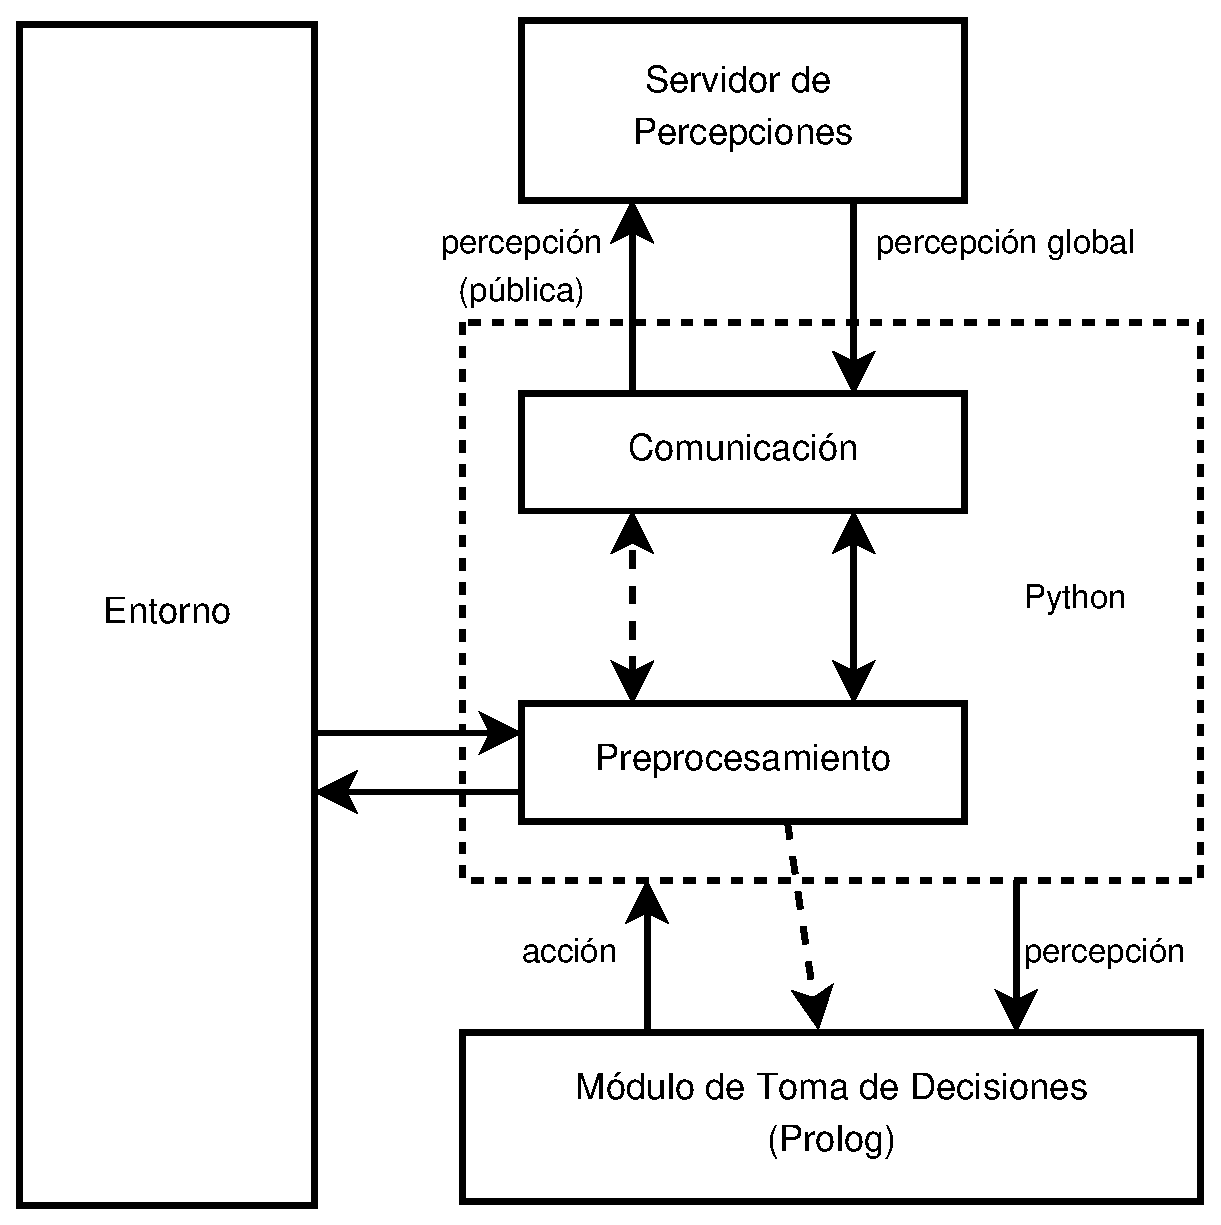
\includegraphics[scale=.4]{graficos/eps/agent_architecture.eps}
 % \caption{Diagrama de la arquitectura del agente. Las líneas punteadas
 % representan el flujo de control, y las líneas contínuas representan el
 % flujo de datos.}
 % \label{fig:architecture}
 % \end{figure}
 
 % El servidor de percepciones (SP) es un programa independiente,
 % encargado de unificar las percepciones de todos los agentes que se
 % encuentran en ejecución.
 % Recibe sus percepciones individuales y retorna a cada uno de ellos el
 % conjunto de datos que aún no poseen, de manera que todos los agentes
 % del equipo cuenten con la misma información en cuanto al estado del
 % escenario.
  
 % En cada iteración de la simulación, el agente recibe un mensaje por
 % parte del servidor del juego, el cual contiene la información
 % asociada a la percepción del turno en disputa.
 % Este mensaje es parseado y traducido en una estructura que permite
 % manipular los datos con mayor facilidad.
 % Los datos son divididos en dos conjuntos, uno ``público'', el cual es
 % compartido con los demás agentes del equipo, y uno ``privado''.
 % La sección pública de datos es compartida a través del mencionado
 % servidor de percepciones.
 
 % El agente une entonces su propia percepción con la percepción global
 % recibida del servidor de percepciones, y genera un único conjunto de
 % datos.
 % Esta información es incorporada a la base de conocimientos,
 % estableciendo nuevas creencias para el agente.
 
 % El módulo de toma de decisiones, analizado en la sección
 % \ref{sec:arquitectura_bdi}, es el que implementa el modelo BDI
 % respetado por el agente.
 % Este módulo es consultado en cada iteración para obtener la próxima
 % acción a ser ejecutada.
 % Una vez que el flujo de control retorna al programa principal, la
 % acción seleccionada es enviada al servidor del juego.
  
\subsubsection{Base de conocimiento}
\label{subsub:base_de_conocimiento}
  
 % Como fue mencionado, la percepción del agente en cada iteración es
 % convertida a una estructura de datos que permite, de manera más
 % sencilla, manipular y compartir la información.
 % Cuando el agente cuenta con todos los datos relativos a las
 % percepciones del equipo, la base de conocimiento puede ser
 % actualizada convenientemente.
 % Una colección de predicados de Prolog consultados desde el programa
 % principal se encarga de verificar que la información existente no
 % resulte sobreescrita, y que información redundante no sea incorporada.
 
 % La información que constituye conocimiento certero sobre el estado del
 % escenario es almacenada mediante términos, que sirven como parámetros
 % del predicado \texttt{k/1} (\textit{knowledge}).
 % Cada uno de los datos de interés es representado mediante un término
 % diferente.
 % En muchos casos, esta clase de términos incluyen un parámetro ligado
 % al número de turno en el cual el dato fue percibido.
 % De esta forma, es posible realizar ciertos análisis, como por
 % ejemplo, considerar obsoleta la información de una determinada
 % antigüedad.
 
 % \begin{verbatim}  
 %   k(equipoAgente(Agente, Equipo)).
 %   k(valorNodo(Nodo, Valor)).
 %   k(arco(Nodo1, Nodo2, Costo)).
 %   k(posicionAgente(Agente, Turno, Posición)).
 %   k(equipoNodo(Turno, Nodo, Dueño)). 
 % \end{verbatim}
 
 % Las creencias que provienen de inferencias y cálculos realizados a
 % partir de información ya existente también son almacenadas mediante
 % términos, en este caso parámetros %argumentos del predicado
 % \texttt{b/1} (\textit{beliefs}). 
 
 % Este tipo de creencias es empleado directamente por el módulo
 % encargado de la toma de decisiones, y se mantienen vigentes sólo
 % durante el turno en el cual fueron generadas. Es decir, que, al
 % finalizar cada turno, son descartadas para evitar futuros problemas o
 % inconcistencias.
 
 % \begin{verbatim}
 %   b(estoyEnLaFrontera).
 %   b(posibleExplorar(Nodo)).
 %   b(haySaboteador(Nodo)).
 % \end{verbatim}
 
 % Existe cierta información que es formulada de manera hipotética.
 % Se trata de datos surgidos de suposiciones realizadas sobre posibles
 % estados futuros del escenario, a partir de su estado actual.
 % Este tipo de datos resulta fundamental para facilitar los cálculos
 % realizados por los algoritmos que se encargan de buscar formas de
 % maximizar el puntaje del equipo.
 % Dado que no constituye información real, sino posible a futuro, se
 % almacena mediante parámetros de un predicado especial, \texttt{h/1}
 % (\textit{hypothetical}).
  
 % \begin{verbatim}
 %   h(nodoEquipo(Nodo, Dueño)).
 %   h(posicion(Turno, Agente, Nodo)). 
 % \end{verbatim}
 
 % Las intenciones surgen del proceso argumentativo explicado más
 % adelante, y son representadas utilizando términos.
 % Si la intención no posee argumentos, entonces es representada mediante
 % un átomo.
 % En otro caso, se emplea un functor que denota el nombre de la
 % intención, acompañado por un argumento.
 % Las acciones, por el contrario, son representadas a través de listas.
 % El primer elemento de la lista es un atómo denotando el tipo de
 % acción.
 % El resto de la lista contiene, ocasionalmente, un término que indica
 % el argumento de la acción, como por ejemplo el nombre de un nodo o un
 % agente.
 % Los planes son representados mediante listas de acciones, es decir,
 % listas de listas.
 
 % Contrario a lo que ocurre con las creencias, tanto las intenciones
 % como los planes constituyen información que debe perdurar en la base
 % de conocimiento tantos turnos como sea necesario.
 % Para este tipo de datos se emplean hechos específicos que cuentan con
 % un único argumento.
 
 % \begin{verbatim}
 %   intencion(explorar(vertex7)).
 %   plan([[recharge], [goto, vertex7], [survey]]).
 % \end{verbatim}
  
%----------------------------------------------------------------BDI-%
\subsection{Arquitectura BDI} 
\label{sub:arquitectura_bdi}

 % El módulo de toma de decisiones es consultado por el programa
 % principal, obtiene la próxima acción a ser ejecutada, y la retorna
 % para que pueda ser enviada.
 % Esta es una secuencia que se reitera en cada uno de los turnos de la
 % simulación, con una característica: cuando es necesario plantear y
 % planificar una nueva meta, intervienen una serie de componentes
 % especiales, que difieren de aquellos involucrados cuando se cuenta con
 % una meta ya planificada.
 % Cada uno de estos componentes es descrito en esta sección.
 
 % \begin{figure}[ht]
 % \centering
 % 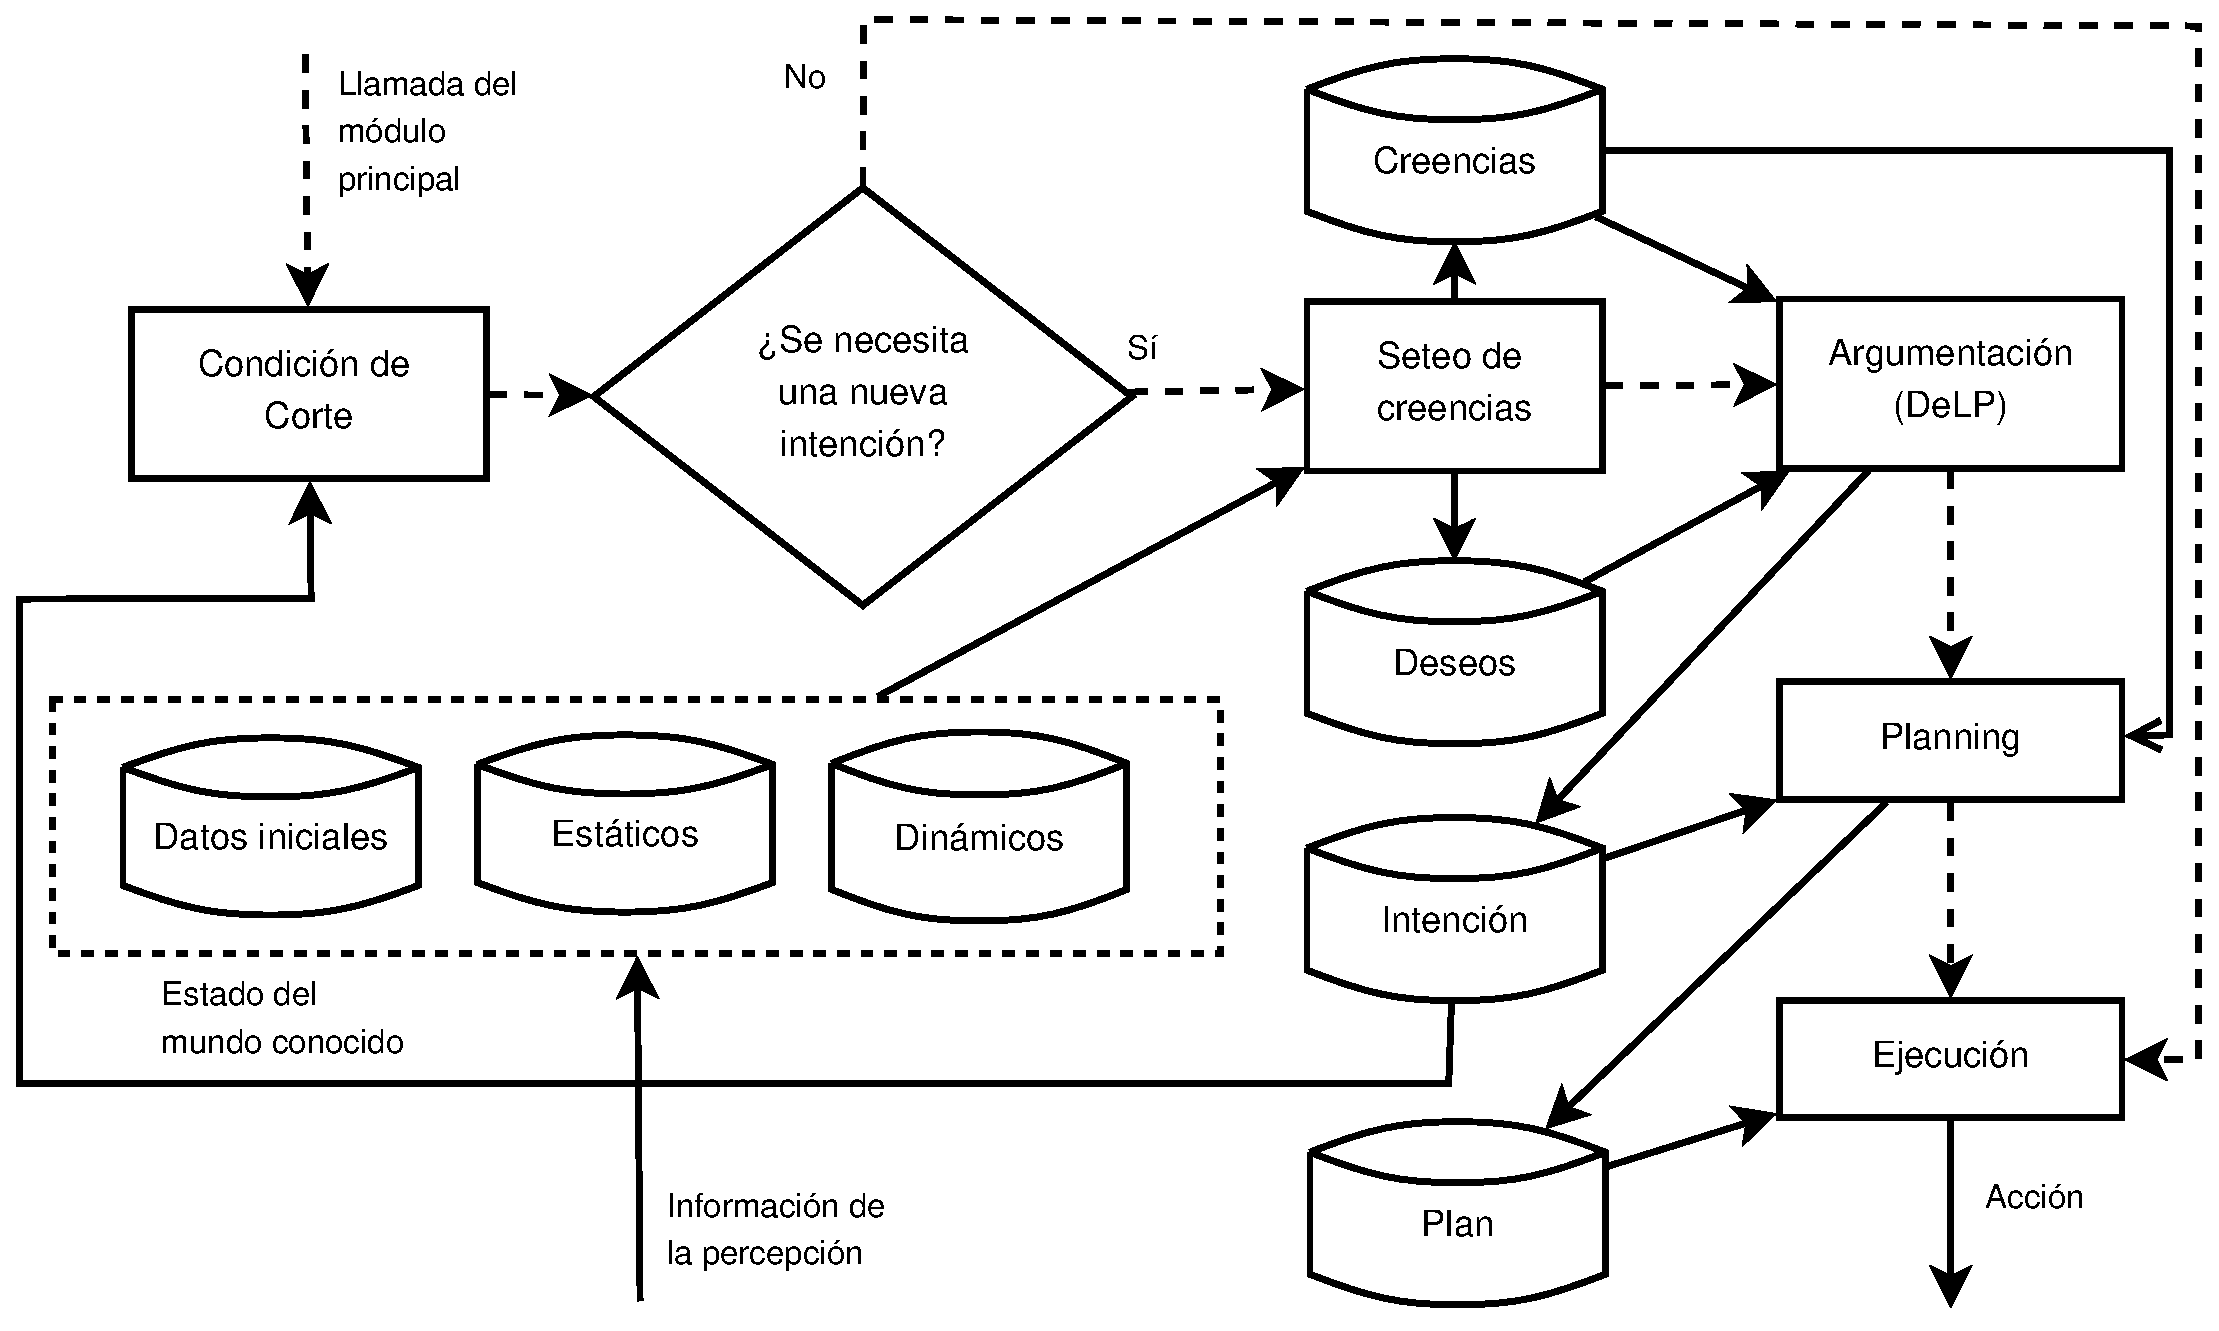
\includegraphics[scale=.3]{graficos/eps/agent_prolog.eps}
 % \caption{Diagrama de la arquitectura interna del agente,
 % particularmente todo lo relacionado con la toma de decisiones, hecha
 % en Prolog.
 % Las líneas punteadas representan el flujo de control, y
 % las líneas contínuas representan el flujo de datos.}
 % \label{fig:agent_prolog}
 % \end{figure}
  
\subsubsection{Seteo de creencias}
\label{subsub:seteo_de_creencias}
  
 % El seteo de creencias es llevado a cabo cada vez que el agente se
 % dispone a seleccionar una nueva intención.
 % Incluye la generación de aquellos datos que pueden permitir al agente
 % realizar una elección lo más acertada posible.
 % Se trata de inferencias realizadas en base al estado del escenario, es
 % decir, aquella información que, como fue mencionado, es almacenada en
 % \texttt{b/1}.
 % No forma parte de este proceso la información proveniente de la
 % percepción, ya que el estado del entorno es actualizado en cada turno
 % de manera previa.
 % Como se detalla a continuación, distintos tipos de creencias pueden
 % pueden estar relacionadas a distintos factores, como el rol del
 % agente, su estado, o los deseos en análisis.
  
 % \paragraph{Creencias generales}
  
 % Existe un conjunto de creencias que resultan de utilidad general para
 % todo el proceso de decisión.
 % Por esta razón, son las primeras en ser calculadas y almacenadas
 % durante el seteo de creencias.
 % Entre los datos incluidos, se encuentra el puntaje que están aportando
 % las zonas armadas, la diferencia de puntos que puede producirse si el
 % agente abandona su posición (ambos puntajes calculados utilizando una
 % versión propia y optimizada del \textit{algoritmo de coloreo} de la
 % competencia, que a su vez será reutilizado en la etapa de resolución
 % de conflictos), y la seguridad que brindan las distintas ubicaciones
 % posibles en cuanto a la presencia de agentes saboteadores enemigos.
  
 % \paragraph{Deseos}
  
 % Como se detallará en la sección siguiente, el proceso de toma de
 % decisión conlleva el pesaje de todos los posibles deseos del agente, y
 % la posterior selección del más beneficioso.
 % Dichos deseos surgen de un conjunto predefinido, y pueden, según sea
 % el caso, estar instanciados con diferentes entidades del juego, como
 % agentes o nodos. Para que esta selección sea posible, es necesario
 % determinar, de manera previa, qué deseos e instanciaciones son
 % realmente factibles, y por lo tanto deben ser tenidos en cuenta, y
 % cuales pueden ser descartados anticipadamente.
 % Para esto se analizan distintas condiciones como, por ejemplo, la
 % distancia a un nodo que no ha sido explorado.
 % Si el nodo se encuentra a una distancia que supera una cota pre-
 % establecida, entonces el deseo de explorar ese nodo no es contemplado.
 % Los deseos e instanciaciones considerados factibles son seteados en la
 % base de conocimiento.
 
 % \begin{verbatim}
 %   b(posibleExplorar(vertex4)).
 % \end{verbatim}
  
 % \paragraph{Creencias específicas} 

 %% Seteo de beliefs para cada deseo.
  
 % Junto con los deseos a ser evaluados, es necesario incluir en la base
 % de conocimiento un conjunto de creencias relacionadas a estos deseos.
 % Entre las más importantes, se encuentran las distancias que existen
 % desde la posición actual del agente a los distintos nodos de interés,
 % y la diferencia de puntaje que se produce en caso que el agente se
 % desplace a dichas ubicaciones.
 % Estos datos resultan fundamentales, ya que afectan directamente la
 % valuación que se realiza de cada deseo, y por lo tanto la posterior
 % selección.
  
 % En esta etapa, también se produce el seteo de datos requeridos
 % posteriormente, como son los caminos a los diferentes nodos
 % analizados.
 % Los algoritmos empleados para la búsqueda de caminos almacenan todos
 % los caminos hallados, en forma de secuencia de acciones, de manera que
 % la etapa de planificación, ejecutada cuando se ha decidido una
 % intención, pueda ser realizada en forma simple e directa.
  
 % \paragraph{Creencias especiales} 

 %% Seteo de beliefs en caso de agente deshabilitado.
  
 % Cuando el agente se encuentra en una situación de peligro, esto es, no
 % posee el rol de saboteador y hay un saboteador enemigo en su posición,
 % o fue atacado en el turno anterior, el conjunto de creencias seteadas
 % se reduce.
 % En estos casos, sólo son tenidos en cuenta los nodos vecinos, dado que
 % representan las vías de escape más rápidas; son calculadas las
 % distancias a estos (en cantidad de turnos), y las diferencias de
 % puntaje que produciría el desplazamiento del agente.
 % Esto tiene el objetivo de minimizar la cantidad de deseos
 % considerados: sólo son evaluadas la posibilidad de permanecer en la
 % misma ubicación (si el beneficio en puntaje es considerable), y las
 % distintas alternativas de defensa propia que pueden llevar al agente a
 % superar el peligro.
  
%------------------------------------------------------ARGUMENTACION-%
\subsection{Argumentación}
\label{sub:argumentacion}
  
 % Una vez finalizado el seteo de creencias, el agente procede a la
 % selección de la próxima intención.
 % Para esto, se toma cada uno de los deseos marcados como factibles en
 % la base de conocimiento, y se los evalua junto a una serie de
 % ``condiciones'' particulares.
 % Se considera que existen razones para creer realizables sólo aquellos
 % deseos que satisfacen sus condiciones.
 % Para estos, se obtiene un valor que representa su peso, en términos
 % del beneficio que conllevan para el equipo.
 % El deseo que presenta el mayor peso entre los analizados, se convierte
 % en la nueva meta del agente, la cual es almacenada hasta ser alcanzada
 % o reemplazada.
 
 % Tanto la evaluación como el pesaje de los deseos, son llevados a cabo
 % empleando \textit{argumentación} en un módulo especial, implementado
 % con la ayuda de \textit{DeLP}.
  
%------------------------------------------------------PLANIFICACION-%
\subsection{Planificación}
\label{sub:planificacion}
  
 % La planificación consiste en obtener la secuencia de acciones que
 % llevan al cumplimiento de la intención propuesta.
 % Esta lista está compuesta por las acciones que le permiten al agente
 % posicionarse en el nodo deseado, y, en algunos casos, una acción
 % concreta a realizar. Como se dijo anteriormente, en la etapa de seteo
 % de creencias, todos los caminos hallados por el algoritmo de búsqueda
 % son almacenados. Dicho algoritmo fue implementado de manera tal que
 % los caminos no están constituidos por nodos o vértices, sino por una
 % secuencia optimal de acciones, que tiene en cuenta no sólo el nodo
 % destino, sino también los recursos del agente, y la meta final a
 % realizar (en caso de haber una acción final).
 % De esta forma, cualquiera haya sido la intención elegida, el agente
 % cuenta en su base de conocimiento con el plan necesario para
 % cumplirla.
 % La planificación se resume entonces a tomar las acciones
 % correspondientes, y establecerlas efectivamente como el plan a seguir.
  
 % Alternativamente, esta etapa puede introducir ciertas acciones con el
 % objetivo de optimizar el uso del turno.
 % En aquellas situaciones en que el agente se dispone a permanecer
 % inactivo, la acción nula (\texttt{skip}) puede ser reemplazada por la
 % acción de recargar energía, si es que esta resulta más productiva.
  
%----------------------------------------------------------EJECUCION-%
\subsection{Ejecución}
\label{sub:ejecucion}
  
 % Dado que el plan se encuentra almacenado de manera completa y
 % ordenada, la ejecución se realiza en forma directa.
 % Se toma la próxima acción, es decir, la primera acción del plan
 % restante, y se la retorna al módulo principal del programa.
 % Éste se encarga posteriormente de enviarla al entorno, para que se
 % convierta finalmente en la siguiente acción realizada por el agente.
  
\subsubsection{Condición de corte}
\label{subsub:condicion_de_corte}
  
 % Existen situaciones en las que el paso de los turnos genera que el
 % cumplimiento de una meta se vuelva inalcanzable, innecesario,
 % riesgoso, o menos productivo de lo previsto, por lo que resulta más
 % beneficioso abortar el plan existente, y seleccionar una nueva
 % intención.
 % Ésta es una etapa de verificación, que tiene como objetivo la
 % detección de este tipo de situaciones.
 % Es ejecutada sólo en aquellos turnos en los que el agente se encuentra
 % siguiendo el plan de una intención previamente determinada.
 
 % Cada deseo o esquema de deseo cuenta con una serie de
 % \textbf{condiciones de corte}, que son evaluadas al inicio de cada
 % turno, en caso de existir un plan establecido.
 % Si se verifica que alguna de estas condiciones se satisface, entonces
 % la intención es descartada, y el agente ingresa en un nuevo proceso de
 % selección. Entre las condiciones de corte tenidas en cuenta, se
 % encuentran:
 
 % \begin{itemize}
 % \item Que haya pasado una determinada cantidad de turnos desde el
 % inicio del plan.
 
 % \item Que el agente se encuentre deshabilitado.
 
 % \item Que haya sido atacado o se encuentre amenazado por un enemigo.
 
 % \item Que la meta haya sido alcanzada por un compañero de equipo.
 % \end{itemize}
  
\subsubsection{Re-planificación}
\label{subsub:replanificacion}
  
 % La fase de re-planificación consiste en elaborar nuevamente el plan
 % que permite alcanzar la meta propuesta, sin modificar dicha meta. Este
 % paso, como el anterior, se realiza en los turnos en los que el agente
 % posee un plan pre-calculado.
 % Dado que en estos turnos no es necesaria la obtención de una nueva
 % intención, proceso que implica el mayor insumo de tiempo, la inclusión
 % de la re-planificación no afecta el funcionamiento normal del agente,
 % en términos de tiempo de ejecución.
 
 % Por el contrario, existe una mejora en el desempeño del equipo,
 % surgida de un mejor aprovechamiento de la información percibida.
 % Los agentes actualizan su información sobre el estado del mundo en
 % cada turno.
 % Datos como el estado en que se hallan los recursos del agente, la
 % incorporación de nodos y arcos hasta el momento desconocidos, o las
 % nuevas ubicaciones de los otros agentes, permiten elaborar planes más
 % precisos y ajustados a la realidad que los originalmente diseñados.
 % Así, los agentes son capaces de cumplir sus metas con mayor facilidad,
 % o abortarlas si es necesario.

